% This is samplepaper.tex, a sample chapter demonstrating the
% LLNCS macro package for Springer Computer Science proceedings;
% Version 2.20 of 2017/10/04
%
\documentclass[runningheads]{llncs}
%
\usepackage{graphicx}
\usepackage{multirow}
\usepackage{adjustbox}
\usepackage{movie15}
\usepackage{float}
\usepackage{longtable}
\usepackage{listings}
\usepackage{amsmath}
\usepackage{systeme}
\usepackage{csquotes}
\usepackage{hyperref}
\hypersetup{
    colorlinks=true, %set true if you want colored links
    linktoc=all,     %set to all if you want both sections and subsections linked
    linkcolor=blue,  %choose some color if you want links to stand out
}
% Used for displaying a sample figure. If possible, figure files should
% be included in EPS format.
%
% If you use the hyperref package, please uncomment the following line
% to display URLs in blue roman font according to Springer's eBook style:
\renewcommand\UrlFont{\color{blue}\rmfamily}

%encoding
%--------------------------------------
\usepackage[T1]{fontenc}
\usepackage[utf8]{inputenc}
%--------------------------------------
%Portuguese-specific commands
%--------------------------------------
\usepackage[portuguese]{babel}
%--------------------------------------
%Hyphenation rules
%--------------------------------------
\usepackage{hyphenat}
\hyphenation{mate-mática recu-perar ma-no equa-ções}

\begin{document}
%
\title{Geração e Resolução de puzzles do tipo \textit{Grape Puzzles}}
%
\titlerunning{Grape Puzzles}
% If the paper title is too long for the running head, you can set
% an abbreviated paper title here
%
\author{Gonçalo Alves\orcidID{up201806451} e
António Bezerra\orcidID{up201806854}}
%
\authorrunning{G. Alves e A. Bezerra}
% First names are abbreviated in the running head.
% If there are more than two authors, 'et al.' is used.
%
\institute{FEUP-PLOG, Turma 3MIEIC03, Grupo Grape\_3\\
\url{https://web.fe.up.pt}}
%
\maketitle              % typeset the header of the contribution
%
\begin{abstract}
Começa-se por definir o objetivo deste trabalho e pela apresentação de informações relevantes sobre cada ponto do trabalho.
De seguida, é descrito o problema \textit{Grape Puzzles} em detalhe.
Na abordagem são descritas: as \textbf{variáveis de decisão} e as \textbf{restrições} aplicadas.
Na secção de visualização da solução são explicados os predicados que permitem diferentes visualizações.
De seguida, são apresentadas as experiências com os respetivos resultados.
Finalmente, são apresentadas as conclusões e o possível trabalho futuro.

\keywords{Grape \and Linhas \and Restrição.}
\end{abstract}
%
%
%
Este artigo descreve o segundo trabalho realizado para a unidade curricular de Programação em Lógica, tendo como objetivo a resolução e geração de problemas do tipo \textit{Grape Puzzles}, através de programação em lógica com restrições.

O problema de decisão \textit{Grape Puzzle} consiste na resolução de \textit{n-1}+...+1 somas, em que as cores representam variáveis iguais. Tomemos o exemplo, do problema seguinte, com 4 linhas:
\begin{figure}
    \centering
    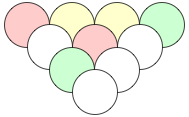
\includegraphics{problem.png}
    \caption{Problema de 4 Linhas}
    \label{fig: 4rowproblem}
\end{figure}

As somas correspondentes, apresentadas de linha a linha, serão:

\begin{equation}
    \systeme*{
    A \+ B = D  &\bigcap B \+ B = A  &\bigcap B \+ C = E ,
    D \+ A = C &\bigcap A \+ E = F,
    C \+ F = G
    }
\end{equation}

Tendo como solução:
\begin{figure}
    \centering
    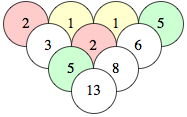
\includegraphics{solution.png}
    \caption{Solução de um problema de 4 Linhas}
    \label{fig: 4rowsolution}
\end{figure}
\section{Abordagem}
\subsection{Variáveis de Decisão}

Tal como descrito na secção anterior, as variáveis de decisão serão os números de cada "uva".
De modo, a representar um \textit{puzzle} como o da Fig.\ref{fig: 4rowproblem}, optou-se por uma lista de listas, em que cada lista representa uma linha do problema.

O predicado \verb|defineDomains/1| é responsável por definir os domínios para cada linha. Inicialmente, atribui à primeira linha o domínio \verb|[1,9]| e depois vai atribuindo às outras listas o domínio \verb|[2,MaxValue]|. A variável \verb|MaxValue| é calculada consoante o número de linhas, através do predicado \verb|defineUpperBound/2|.

\subsection{Restrições}
As restrições deste problema são as seguintes:
\begin{itemize}
    \item Primeira linha apenas pode conter números positivos de um dígito
    \item A "uva" que se encontra debaixo de duas "uvas" é a soma destas
    \item "Uvas" com a mesma cor, contêm o mesmo número, com excepção da cor branca
    \item Há um número máximo de cores
\end{itemize}

As três primeiras restrições do problema são restrições rígidas.
A última restrição foi assumida pelo grupo e isto deve-se ao facto de não estar presente no enunciado qualquer tipo de indicação sobre o número de cores obrigatórias que o problema deve ter. Assim, criou-se esta restrição flexível para poder gerar problemas inferiores a 4 linhas (problemas de 2 linhas não conseguiriam ter 3 cores) e problemas superiores a 6 linhas (problemas maiores vão necessitar de mais cores para não se tornarem demasiado difíceis para quem os está a resolver).

Assim, para a primeira restrição fez-se uso do predicado \verb|domain/3| da biblioteca \textbf{clpfd} do SICStus para limitar o domínio, como referido na subsecção anterior.
Para a restrição da soma, desenvolveu-se o predicado \verb|defineSumConstraints/1|, que percorre as listas e coloca a restrição \verb|FirstUpper + SecondUpper #= Child|, para cada linha após a primeira.
Por fim, a restrição de cor é feita com recurso ao predicado \verb|global_cardinality/2|. Numa primeira fase, este predicado permite contar o número de ocorrências de números numa lista e com uma segunda chamada deste predicado, é possível restringir a ocorrência de pares de números ao número de cores necessárias.

\section{Visualização da Solução}
De modo a visualizar o "cacho de uvas" e tornar a experiência do utilizador mais apelativa, foram criados dois predicados \verb|displayOutput/2| e \verb|displayOutput/3|, que apresentam a solução e o puzzle seguido da solução, respetivamente.

A primeira versão do predicado apenas apresenta a solução do problema e é utilizada no predicado \verb|grapesolver/1|.

A segunda versão apresenta tanto o problema, com as cores substituidas por letras, como a solução respetiva. Esta versão é utilizada no predicado \verb|grapegenerator/2|.

\begin{figure}
    \centering
    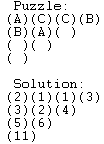
\includegraphics{print.png}
    \caption{Impressão de Resultados}
    \label{fig: results}
\end{figure}
\section{Experiências e Resultados}
O programa foi testado de modo a ser possível estudar o comportamento da nossa resolução não só com puzzles de tamanho diferente, mas também com estratégias de pesquisa diferentes.
É de salientar que os resultados apresentados poderão diferir de máquina para máquina, devido aos diferentes tempos de processamento.

\subsection{Análise Dimensional}
O programa foi testado com problemas de 2 a 7 linhas.

\begin{table}[h!]
\centering
\begin{tabular}{|c|c|c|} 
 \hline
 Número de Linhas & Tempo de Execução (s) & Número de Soluções \\ [0.5ex] 
 \hline
 2 & 0 & 9  \\
 3 & 0.015 & 80 \\
 4 & 0.125 & 240 \\
 5 & 1.438 & 9854 \\
 6 & 13.906 & 96134 \\
 7 & 128.641 & 212350 \\ [1ex] 
 \hline
\end{tabular}
\caption{Resultados de uma Análise Dimensional}
\label{table: dimensional_analisys}
\end{table}

Como podemos observar pela tabela acima e pelos gráficos respetivos [\ref{fig: sizegraph},\ref{fig: sizeresultsgraph}], o crescimento do tempo e das soluções encontradas foi exponencial. Por esta razão, não se testaram problemas de tamanho superior a 7 linhas.

Devido à falta de tempo, não foi possível desenvolver uma restrição que nos permitisse remover puzzles "espelhados", ver Fig \ref{fig: originalproblem} e \ref{fig: invertedproblem}.


\subsection{Estratégias de Pesquisa}
O programa foi testado com todas as combinações de heurísticas, para problemas de 5 linhas.

\begin{table}[h!]
\centering
\resizebox{9cm}{!}{
\begin{tabular}{|c|c|c|c|} 
 \hline
Ordenação de Variáveis & Seleção de Valores &  Ordenação de Valores & Tempo de Execução (s)\\ [0.5ex] 
 \hline
\multirow{5}{*}{leftmost} & \multirow{2}{*}{step} & up & 2.422 \\ 
                            &                         & down & 2.563 \\
                            & \multirow{2}{*}{enum} & up & 1.531 \\ 
                            &                         & down & 1.531 \\
                            & \multirow{2}{*}{bisect} & up & 1.875 \\ 
                            &                         & down & 2.047 \\
                            & \multirow{2}{*}{median} & up & 2.469 \\ 
                            &                         & down & 2.547 \\
                            & \multirow{2}{*}{middle} & up & 2.422 \\ 
                            &                         & down & 2.578 \\
 \hline
\multirow{5}{*}{min} & \multirow{2}{*}{step} & up & 2.656 \\ 
                            &                         & down & 2.594 \\
                            & \multirow{2}{*}{enum} & up & 1.547 \\ 
                            &                         & down & 1.578 \\
                            & \multirow{2}{*}{bisect} & up & 2.453 \\ 
                            &                         & down & 2.531 \\
                            & \multirow{2}{*}{median} & up & 2.656 \\ 
                            &                         & down & 2.594 \\
                            & \multirow{2}{*}{middle} & up & 2.656 \\ 
                            &                         & down & 2.594 \\
 \hline
\multirow{5}{*}{max} & \multirow{2}{*}{step} & up & 3.156 \\ 
                            &                         & down & 3.782 \\
                            & \multirow{2}{*}{enum} & up & 1.875 \\ 
                            &                         & down & 1.89 \\
                            & \multirow{2}{*}{bisect} & up & 3.203 \\ 
                            &                         & down & 3.172 \\
                            & \multirow{2}{*}{median} & up & 3.266 \\ 
                            &                         & down & 3.828 \\
                            & \multirow{2}{*}{middle} & up & 3.219 \\ 
                            &                         & down & 3.781 \\
 \hline
\multirow{5}{*}{ff} & \multirow{2}{*}{step} & up & 2.438 \\ 
                            &                         & down & 2.562 \\
                            & \multirow{2}{*}{enum} & up & 1.516 \\ 
                            &                         & down & 1.547 \\
                            & \multirow{2}{*}{bisect} & up & 1.89 \\ 
                            &                         & down & 2.016 \\
                            & \multirow{2}{*}{median} & up & 2.453 \\ 
                            &                         & down & 2.578 \\
                            & \multirow{2}{*}{middle} & up & 2.453 \\ 
                            &                         & down & 2.578 \\
 \hline
\multirow{5}{*}{anti\_first\_fail} & \multirow{2}{*}{step} & up & 12.672 \\ 
                            &                         & down & 11.078 \\
                            & \multirow{2}{*}{enum} & up & 5.157 \\ 
                            &                         & down & 5.187 \\
                            & \multirow{2}{*}{bisect} & up & 6.125 \\ 
                            &                         & down & 6.297 \\
                            & \multirow{2}{*}{median} & up & 12.781 \\ 
                            &                         & down & 11.156 \\
                            & \multirow{2}{*}{middle} & up & 12.735 \\ 
                            &                         & down & 11.203 \\
 \hline
\multirow{5}{*}{occurrence} & \multirow{2}{*}{step} & up & 2.406 \\ 
                            &                         & down & 2.485 \\
                            & \multirow{2}{*}{enum} & up & 1.485 \\ 
                            &                         & down & 1.5 \\
                            & \multirow{2}{*}{bisect} & up & 1.828 \\ 
                            &                         & down & 1.922 \\
                            & \multirow{2}{*}{median} & up & 2.343 \\ 
                            &                         & down & 2.438 \\
                            & \multirow{2}{*}{middle} & up & 2.344 \\ 
                            &                         & down & 2.453 \\
 \hline
\multirow{5}{*}{ffc} & \multirow{2}{*}{step} & up & 2.359 \\ 
                            &                         & down & 2.453 \\
                            & \multirow{2}{*}{enum} & up & 1.469 \\ 
                            &                         & down & 1.516 \\
                            & \multirow{2}{*}{bisect} & up & 1.796 \\ 
                            &                         & down & 1.954 \\
                            & \multirow{2}{*}{median} & up & 2.375 \\ 
                            &                         & down & 2.515 \\
                            & \multirow{2}{*}{middle} & up & 2.344 \\ 
                            &                         & down & 2.484 \\
 \hline
\multirow{5}{*}{max_regret} & \multirow{2}{*}{step} & up & 2.5 \\ 
                            &                         & down & 2.672 \\
                            & \multirow{2}{*}{enum} & up & 1.578 \\ 
                            &                         & down & 1.61 \\
                            & \multirow{2}{*}{bisect} & up & 1.922 \\ 
                            &                         & down & 2.031 \\
                            & \multirow{2}{*}{median} & up & 2.484 \\ 
                            &                         & down & 2.703 \\
                            & \multirow{2}{*}{middle} & up & 2.469 \\ 
                            &                         & down & 2.656 \\
 \hline
\end{tabular}
}
\caption{Resultados de diferentes Estratégias de Pesquisa}
\label{table: search_analisys}
\end{table}
Através da observação da tabela seguinte e do respetivo gráfico  [\ref{fig: searchstrategy}] , concluímos que a combinação mais eficiente seria \textbf{[ffc,enum,up]}.
\section{Conclusão e Trabalho Futuro}
Este trabalho permitiu-nos aprender uma nova metodologia de programar, muito diferente e mais eficaz do que a abordagem tradicional de \textit{Generate\&Test}. Além disso, ficámos cientes da utilidade de programação em lógica com restrições, no mundo real.

Quanto a trabalho futuro, gostaríamos de melhorar a restrição flexível do número de cores e para além disso, realizar mais testes. Devido à falta de tempo, não conseguimos pensar numa relação entre o tamanho do problema e o número de cores e não conseguimos desenvolver a restrição de para análise dimensional referida na secção respetiva.
\begin{thebibliography}{8}

\bibitem{ref_url1}
\textit{Grape Puzzles}, \url{https://erich-friedman.github.io/puzzle/grapes/}. Last accessed 3
Jan 2021
\end{thebibliography}
\appendix
\section{Gráficos}

\begin{figure}
    \centering
    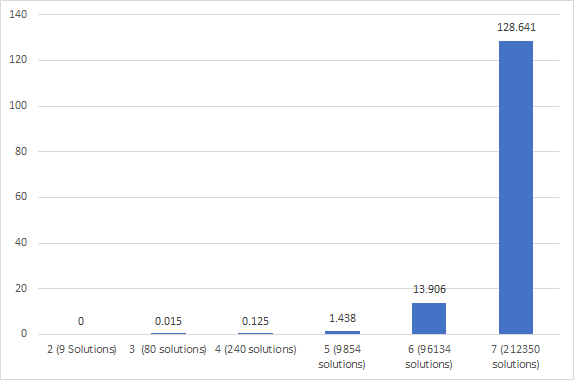
\includegraphics[scale=0.9]{sizes.png}
    \caption{Tempos de execução por Número de linhas do problema}
    \label{fig: sizegraph}
\end{figure}

\begin{figure}
    \centering
    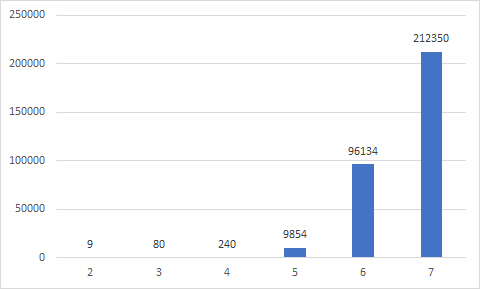
\includegraphics[scale=1.1]{solutions.png}
    \caption{Número de soluções por Número de linhas do problema}
    \label{fig: sizeresultsgraph}
\end{figure}

\begin{figure}
    \centering
    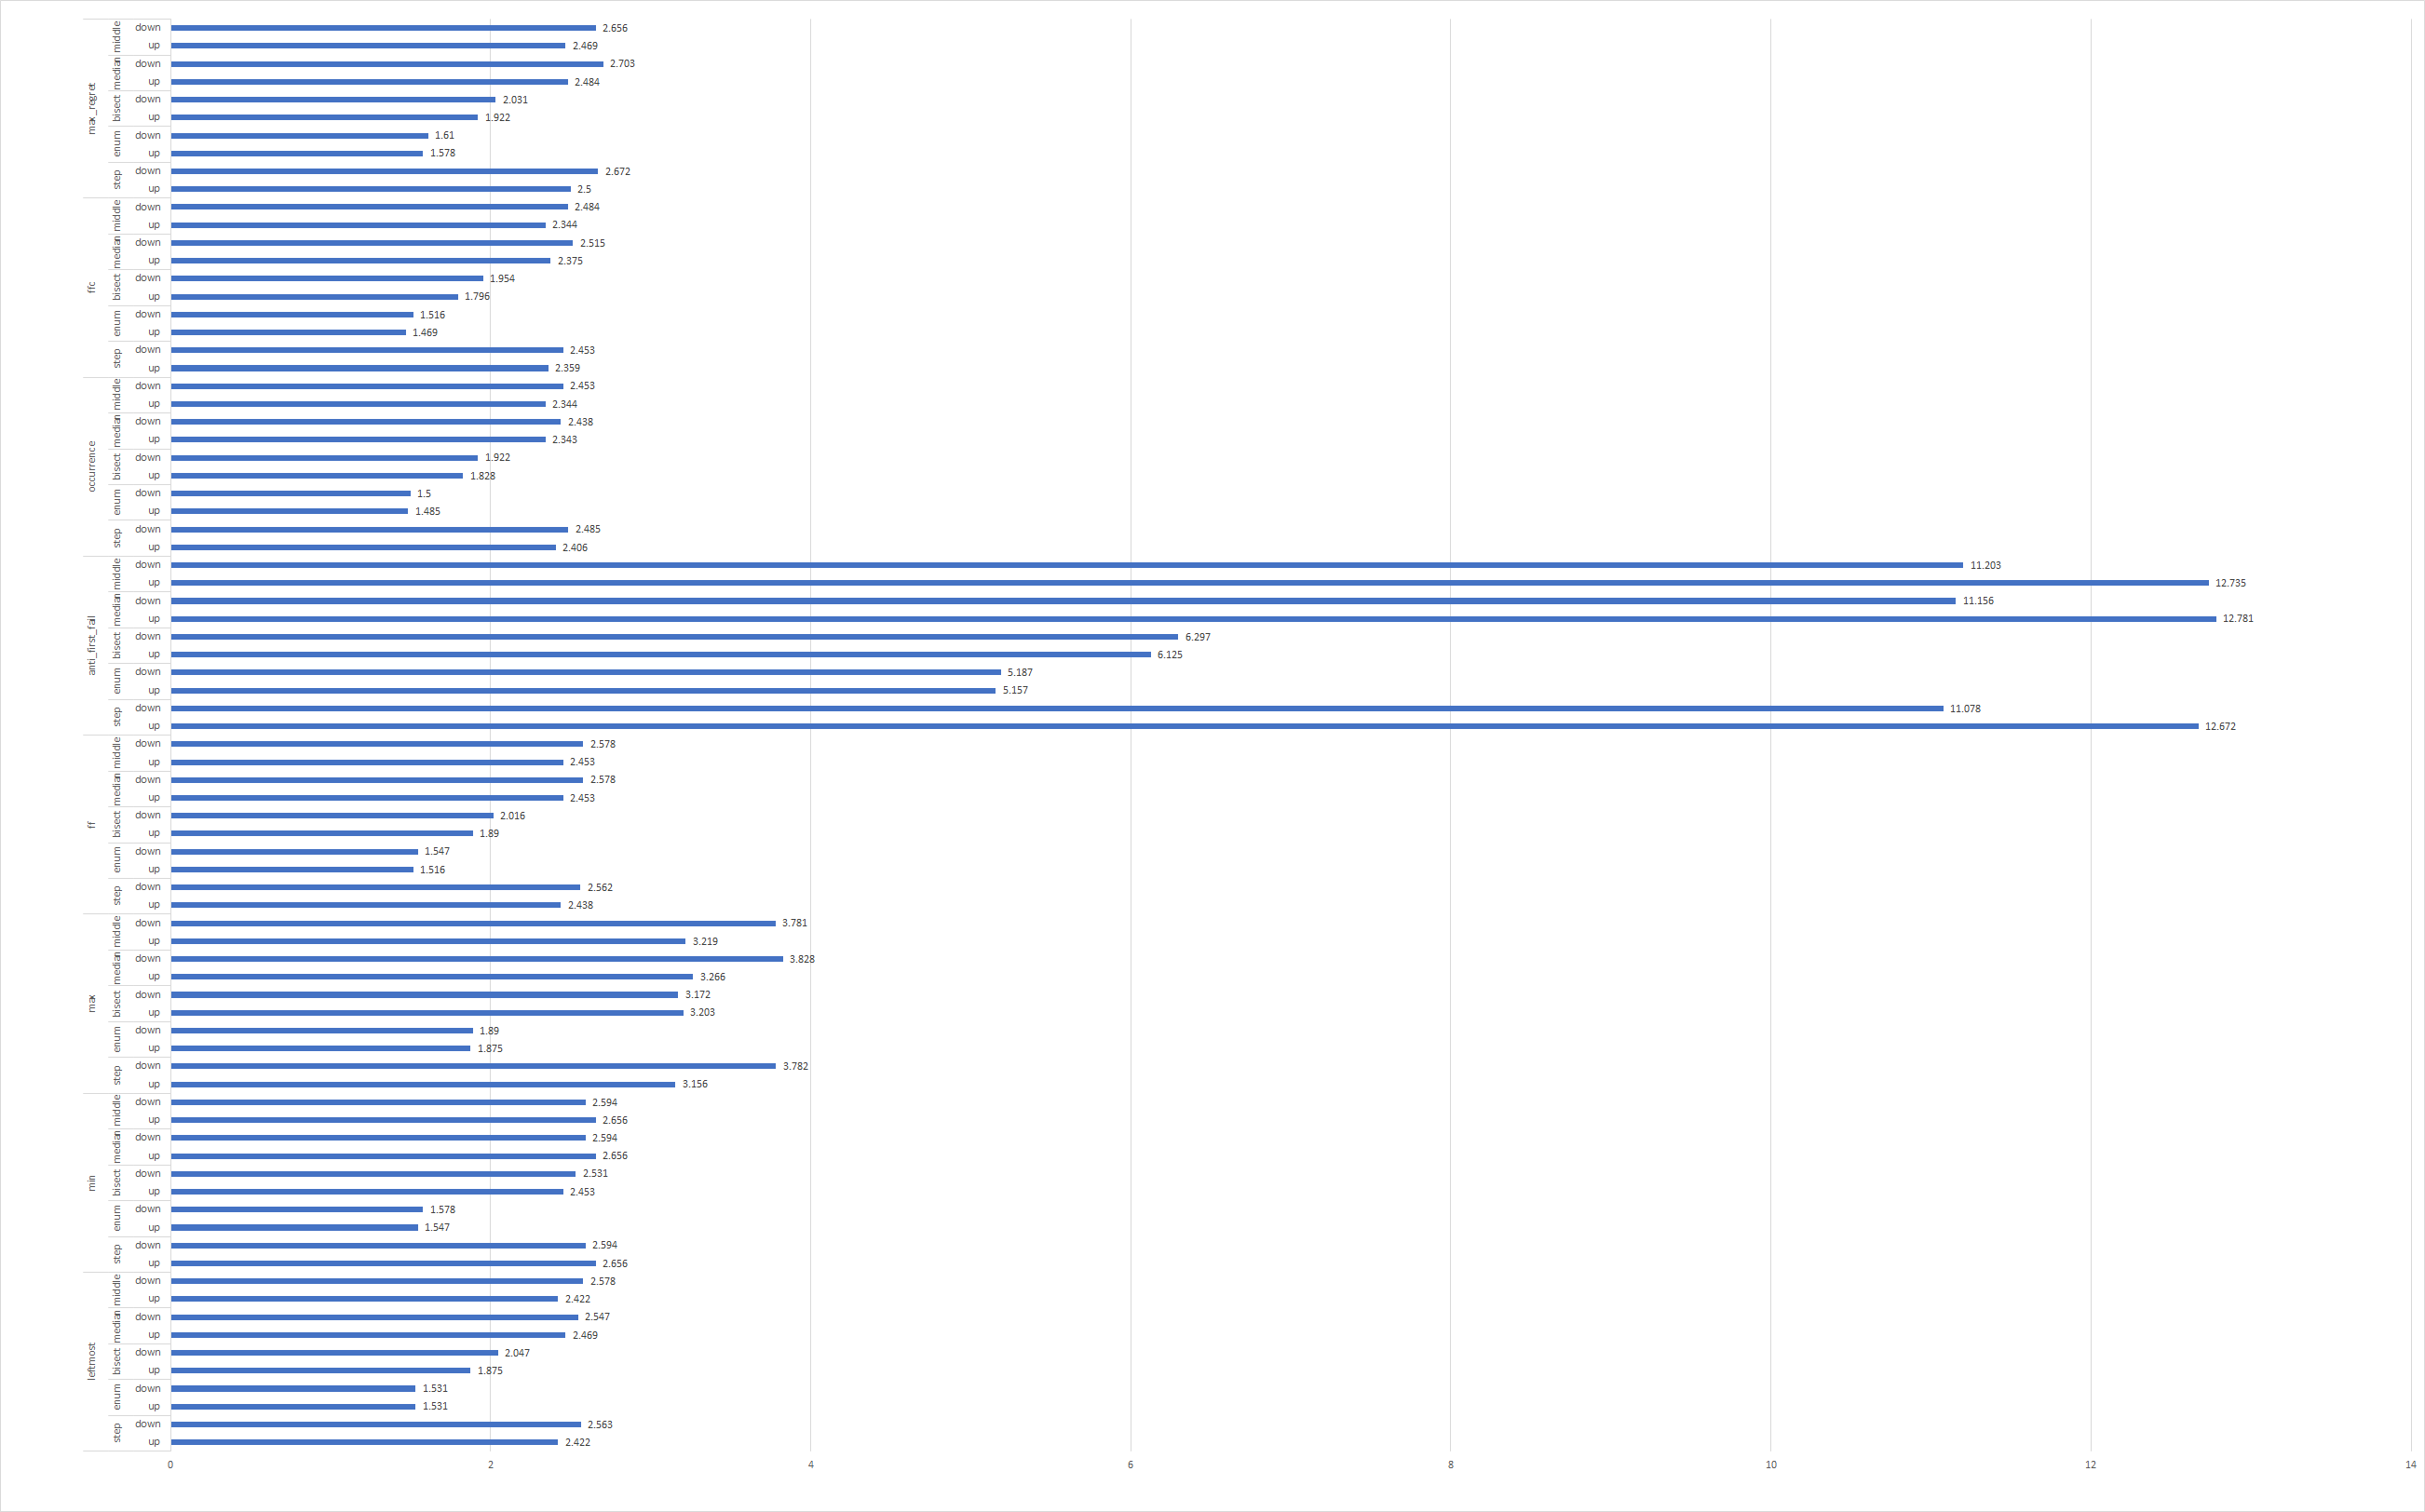
\includegraphics[angle=-90,scale=0.3]{heuristics.png}
    \caption{Análise temporal de estratégias de pesquisa, para um problema de 5 linhas}
    \label{fig: searchstrategy}
\end{figure}
\clearpage
\section{Imagens}

\begin{figure}[!htb]
    \centering
    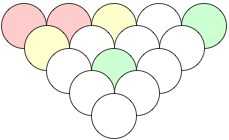
\includegraphics{puzzle.png}
    \caption{Problema original}
    \label{fig: originalproblem}
\end{figure}

\begin{figure}[!htb]
    \centering
    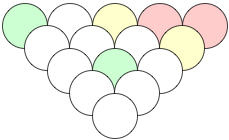
\includegraphics{puzzle_inverted.png}
    \caption{Problema invertido}
    \label{fig: invertedproblem}
\end{figure}



\end{document}
